\documentclass[12pt,a4paper]{article}

\usepackage[margin=1in]{geometry}
\usepackage{amsmath,amssymb}
\usepackage{booktabs}
\usepackage{enumitem}
\usepackage{setspace}
\usepackage{fancyhdr}
\usepackage{hyperref}
\usepackage{xcolor}
\usepackage{listings}
\usepackage{tikz}
\usetikzlibrary{arrows.meta,positioning,shapes.geometric,shadows}

% ----- colors -----
\definecolor{cBlue}{RGB}{66,133,244}
\definecolor{cGreen}{RGB}{52,168,83}
\definecolor{cOrange}{RGB}{251,188,5}
\definecolor{cRed}{RGB}{234,67,53}
\definecolor{cPurple}{RGB}{156,39,176}
\definecolor{cTeal}{RGB}{0,150,136}
\definecolor{cCodeBg}{RGB}{248,249,250}
\definecolor{cCodeKw}{RGB}{0,102,153}
\definecolor{cCodeStr}{RGB}{163,21,21}
\definecolor{cCodeCmt}{RGB}{0,128,0}

\hypersetup{colorlinks=true, linkcolor=black, urlcolor=blue}
\onehalfspacing
\setlength{\parskip}{0.4em}
\setlength{\parindent}{0pt}

\pagestyle{fancy}
\fancyhf{}
\fancyhead[L]{\small Cryptographic Systems Project}
\fancyhead[R]{\small Cryptography \& Network Security}
\fancyfoot[C]{\thepage}
\setlength{\headheight}{14pt}

% ----- code style -----
\lstset{
  language=JavaScript,
  basicstyle=\ttfamily\small,
  keywordstyle=\color{cCodeKw}\bfseries,
  stringstyle=\color{cCodeStr},
  commentstyle=\color{cCodeCmt}\itshape,
  backgroundcolor=\color{cCodeBg},
  frame=single,
  rulecolor=\color{black!20},
  breaklines=true,
  showstringspaces=false,
  tabsize=2,
  numbers=left,
  numberstyle=\tiny\color{gray},
  numbersep=6pt,
  xleftmargin=1.5em,
  framexleftmargin=1em,
  morekeywords={const,let,of,export,function,return,null,true,false,throw,Error}
}

% ----- tikz box styles -----
\newcommand{\flowarrow}{-{Stealth}, thick, color=black!60}

\begin{document}

% ===================== TITLE PAGE =====================
\begin{titlepage}
\centering
\vspace*{1.2cm}

{\Large \textbf{Metropolitan University}}\\[0.3cm]
{\large Department of Computer Science and Engineering}\\[1.2cm]

{\large Project Report}\\[0.4cm]
{\LARGE \textbf{Classical Cryptographic Systems}}\\[0.3cm]
{\large Caesar, Vigen\`{e}re, Playfair, and Hill Cipher Tools}\\[0.6cm]
{\large Course: Cryptography and Network Security}\\[1.8cm]

\begin{tabular}{ll}
\toprule
\textbf{Team Members} & \textbf{Registration No.} \\
\midrule
Ruma Akter & 2021331525 \\
Toufik Islam & 2021331538 \\
Saiful Islam & 2021331541 \\
Nishad Mahmud & 2021331560 \\
\bottomrule
\end{tabular}

\vspace{1.8cm}

\begin{tabular}{ll}
\textbf{Submitted to:} & Golam Mostofa Naeem \\
 & Lecturer, CSE, Metropolitan University \\
\end{tabular}

\vfill
{\large \today}
\end{titlepage}

\tableofcontents
\newpage

% ===================== 1 =====================
\section{Introduction}

For our Cryptography and Network Security course project, we built a small set of web tools that encrypt and decrypt text using four classical ciphers:

\begin{itemize}[leftmargin=*]
  \item Caesar cipher
  \item Vigen\`{e}re cipher
  \item Playfair cipher
  \item Hill cipher
\end{itemize}

Each tool is a simple page with:
\begin{itemize}[leftmargin=*]
  \item a text input box
  \item a key field (shift, keyword, or matrix)
  \item Encrypt / Decrypt mode switch
  \item live output
  \item a demo button with sample data
\end{itemize}

All logic runs in the browser using JavaScript. Nothing is sent to a server for encryption. The goal was to turn the ciphers we studied in class into working tools we can actually use and show.

\section{Objectives}

\begin{enumerate}[leftmargin=*]
  \item Implement four classical ciphers in JavaScript.
  \item Build a simple UI for each cipher (input, key, mode, output).
  \item Handle real text (spaces, punctuation, case) in a sensible way.
  \item For Hill, support a general \(n \times n\) key matrix (invertible mod~26).
  \item Add demo examples so anyone can try the tools quickly.
\end{enumerate}

% ===================== 2 =====================
\section{How the Project Works}

We kept the same pattern for every cipher:

\begin{enumerate}[leftmargin=*]
  \item Put the math / cipher logic in a small JS module (for example \texttt{caesar.js}).
  \item Export \texttt{encrypt()} and \texttt{decrypt()} functions.
  \item Connect those functions to a React page with input fields.
  \item When the user types or changes the mode, the page calls the function and shows the result.
\end{enumerate}

\begin{center}
\begin{tikzpicture}[
  node distance=0.85cm and 0.9cm,
  box/.style={draw, rounded corners=3pt, align=center, minimum width=2.7cm,
              minimum height=1.15cm, font=\small\bfseries, drop shadow={shadow xshift=0.6pt, shadow yshift=-0.6pt, opacity=0.2}},
  arrow/.style={\flowarrow}
]
  \node[box, fill=cBlue!25, draw=cBlue] (ui) {Web UI\\(input + key)};
  \node[box, fill=cOrange!35, draw=cOrange, right=of ui] (mode) {Encrypt\\or Decrypt};
  \node[box, fill=cPurple!25, draw=cPurple, right=of mode] (js) {JS cipher\\module};
  \node[box, fill=cGreen!30, draw=cGreen, right=of js] (out) {Show\\output};

  \draw[arrow] (ui) -- (mode);
  \draw[arrow] (mode) -- (js);
  \draw[arrow] (js) -- (out);
\end{tikzpicture}
\end{center}

Figure above: one shared flow for all four tools. Only the middle ``JS cipher module'' changes per cipher.

% ===================== 3 =====================
\section{Caesar Cipher}

\subsection{What we built}
The Caesar tool shifts every letter by a number \(k\). Spaces, digits, and punctuation stay unchanged. Uppercase and lowercase are handled separately so case is preserved.

\begin{itemize}[leftmargin=*]
  \item Encrypt: \(C = (P + k) \bmod 26\)
  \item Decrypt: \(P = (C - k) \bmod 26\)
\end{itemize}

\subsection{Flow diagram}
\begin{center}
\begin{tikzpicture}[
  node distance=0.5cm,
  box/.style={draw, rounded corners=3pt, align=center, minimum width=8.2cm,
              minimum height=0.9cm, font=\small, drop shadow={shadow xshift=0.5pt, shadow yshift=-0.5pt, opacity=0.18}},
  arrow/.style={\flowarrow}
]
  \node[box, fill=cBlue!20, draw=cBlue] (a) {1. Take input text + shift \(k\)};
  \node[box, fill=cTeal!20, draw=cTeal, below=of a] (b) {2. For each character: if letter \(\rightarrow\) shift by \(k\) or \(-k\)};
  \node[box, fill=cOrange!25, draw=cOrange, below=of b] (c) {3. Keep spaces / digits / punctuation as-is};
  \node[box, fill=cGreen!25, draw=cGreen, below=of c] (d) {4. Return encrypted or decrypted text};
  \draw[arrow] (a) -- (b);
  \draw[arrow] (b) -- (c);
  \draw[arrow] (c) -- (d);
\end{tikzpicture}
\end{center}

\subsection{Example}
\begin{center}
\begin{tabular}{@{}cccc@{}}
\toprule
Letter & Number & \(+3 \bmod 26\) & Result \\
\midrule
H & 7 & 10 & K \\
E & 4 & 7 & H \\
L & 11 & 14 & O \\
L & 11 & 14 & O \\
O & 14 & 17 & R \\
\bottomrule
\end{tabular}
\end{center}
So \texttt{HELLO} with shift \(3\) becomes \texttt{KHOOR}.

\subsection{JavaScript code (main part)}
\begin{lstlisting}
function transform(text, shift) {
  const s = ((shift % 26) + 26) % 26;
  let out = "";
  for (const ch of text) {
    const code = ch.charCodeAt(0);
    const isUpper = code >= 65 && code <= 90;
    const isLower = code >= 97 && code <= 122;
    if (!isUpper && !isLower) {
      out += ch;           // leave non-letters
      continue;
    }
    const base = isUpper ? 65 : 97;
    const idx = code - base;
    out += String.fromCharCode(base + ((idx + s) % 26));
  }
  return out;
}

export function encrypt(text, shift) {
  return transform(text, shift);
}
export function decrypt(text, shift) {
  return transform(text, -shift);
}
\end{lstlisting}

\subsection{UI features}
\begin{itemize}[leftmargin=*]
  \item Shift can be any integer (we take it mod~26).
  \item Demo loads: \texttt{Attack at dawn!} with shift \(3\).
  \item User can switch Encrypt \(\leftrightarrow\) Decrypt and reuse the output as input.
\end{itemize}

% ===================== 4 =====================
\section{Vigen\`{e}re Cipher}

\subsection{What we built}
Vigen\`{e}re uses a keyword. The keyword repeats and each letter of the message gets a different shift from the matching keyword letter. Non-letters stay in place and do not move the keyword pointer forward.

\begin{itemize}[leftmargin=*]
  \item Keyword is cleaned to letters A--Z only.
  \item Encrypt: add keyword shift \(\bmod 26\)
  \item Decrypt: subtract keyword shift \(\bmod 26\)
\end{itemize}

\subsection{Flow diagram}
\begin{center}
\begin{tikzpicture}[
  node distance=0.5cm,
  box/.style={draw, rounded corners=3pt, align=center, minimum width=8.6cm,
              minimum height=0.9cm, font=\small, drop shadow={shadow xshift=0.5pt, shadow yshift=-0.5pt, opacity=0.18}},
  arrow/.style={\flowarrow}
]
  \node[box, fill=cBlue!20, draw=cBlue] (a) {1. Input text + keyword};
  \node[box, fill=cPurple!20, draw=cPurple, below=of a] (b) {2. Clean keyword (A--Z only)};
  \node[box, fill=cTeal!20, draw=cTeal, below=of b] (c) {3. For each letter: shift using next keyword letter};
  \node[box, fill=cOrange!25, draw=cOrange, below=of c] (d) {4. Skip non-letters (do not advance keyword)};
  \node[box, fill=cGreen!25, draw=cGreen, below=of d] (e) {5. Return result};
  \draw[arrow] (a) -- (b);
  \draw[arrow] (b) -- (c);
  \draw[arrow] (c) -- (d);
  \draw[arrow] (d) -- (e);
\end{tikzpicture}
\end{center}

\subsection{Example}
Plaintext: \texttt{ATTACK}, keyword: \texttt{LEMON}

\begin{center}
\begin{tabular}{@{}ccccc@{}}
\toprule
Plain & \(P\) & Key & \(K\) & Cipher \\
\midrule
A & 0 & L & 11 & L \\
T & 19 & E & 4 & X \\
T & 19 & M & 12 & F \\
A & 0 & O & 14 & O \\
C & 2 & N & 13 & P \\
K & 10 & L & 11 & V \\
\bottomrule
\end{tabular}
\end{center}
Result starts with \texttt{LXFOPV}.

\subsection{JavaScript code (main part)}
\begin{lstlisting}
function normalizeKey(key) {
  return (key || "").toUpperCase().replace(/[^A-Z]/g, "");
}

function transform(text, key, isDecrypt) {
  const k = normalizeKey(key);
  if (!k) return "";
  let out = "", ki = 0;
  for (const ch of text) {
    const code = ch.charCodeAt(0);
    const isLetter =
      (code >= 65 && code <= 90) || (code >= 97 && code <= 122);
    if (!isLetter) { out += ch; continue; }

    const base = code <= 90 ? 65 : 97;
    const idx = code - base;
    const kShift = k.charCodeAt(ki % k.length) - 65;
    const shift = isDecrypt ? -kShift : kShift;
    out += String.fromCharCode(base + ((idx + shift + 260) % 26));
    ki++;
  }
  return out;
}
\end{lstlisting}

\subsection{UI features}
\begin{itemize}[leftmargin=*]
  \item Demo: plaintext \texttt{Attack at dawn!}, key \texttt{LEMON}.
  \item Empty keyword \(\rightarrow\) no output (invalid key).
  \item Spaces and punctuation stay visible in the result.
\end{itemize}

% ===================== 5 =====================
\section{Playfair Cipher}

\subsection{What we built}
Playfair encrypts letters in pairs using a \(5\times5\) square built from a keyword. We merge \(I\) and \(J\). If two letters in a pair are the same, we insert \(X\). A leftover single letter is padded with \(X\).

Rules we coded:
\begin{itemize}[leftmargin=*]
  \item Same row \(\rightarrow\) take the letters to the right (wrap around)
  \item Same column \(\rightarrow\) take the letters below (wrap around)
  \item Rectangle \(\rightarrow\) swap the column of each letter
\end{itemize}
Decrypt uses left / up instead of right / down.

\subsection{Flow diagram}
\begin{center}
\begin{tikzpicture}[
  node distance=0.5cm,
  box/.style={draw, rounded corners=3pt, align=center, minimum width=8.8cm,
              minimum height=0.9cm, font=\small, drop shadow={shadow xshift=0.5pt, shadow yshift=-0.5pt, opacity=0.18}},
  arrow/.style={\flowarrow}
]
  \node[box, fill=cBlue!20, draw=cBlue] (a) {1. Input text + keyword};
  \node[box, fill=cPurple!20, draw=cPurple, below=of a] (b) {2. Build \(5\times5\) square from keyword};
  \node[box, fill=cTeal!20, draw=cTeal, below=of b] (c) {3. Split into digraphs (insert \(X\) if needed)};
  \node[box, fill=cOrange!25, draw=cOrange, below=of c] (d) {4. Apply row / column / rectangle rule};
  \node[box, fill=cRed!15, draw=cRed, below=of d] (e) {5. Join pairs and return ciphertext};
  \draw[arrow] (a) -- (b);
  \draw[arrow] (b) -- (c);
  \draw[arrow] (c) -- (d);
  \draw[arrow] (d) -- (e);
\end{tikzpicture}
\end{center}

\subsection{Example}
Keyword: \texttt{MONARCHY}. Demo plaintext: \texttt{INSTRUMENTS}.

Sample square (I/J merged):
\[
\begin{bmatrix}
M & O & N & A & R \\
C & H & Y & B & D \\
E & F & G & I/J & K \\
L & P & Q & S & T \\
U & V & W & X & Z
\end{bmatrix}
\]

\subsection{JavaScript code (main part)}
\begin{lstlisting}
function buildSquare(key) {
  // unique keyword letters, then fill rest of alphabet (no J)
  const k = normalizeKey(key);
  let alpha = "";
  const seen = new Set(k.split(""));
  for (let i = 0; i < 26; i++) {
    const ch = String.fromCharCode(65 + i);
    if (ch === "J" || seen.has(ch)) continue;
    alpha += ch;
  }
  const square = (k + alpha).slice(0, 25);
  // ... also store position map for each letter
  return { square /*, pos */ };
}

function chunkDigraphs(text) {
  const cleaned = text.toUpperCase()
    .replace(/[^A-Z]/g, "").replace(/J/g, "I");
  const pairs = [];
  let i = 0;
  while (i < cleaned.length) {
    const a = cleaned[i], b = cleaned[i + 1];
    if (!b) { pairs.push([a, "X"]); break; }
    if (a === b) { pairs.push([a, "X"]); i++; }
    else { pairs.push([a, b]); i += 2; }
  }
  return pairs;
}
\end{lstlisting}

For each digraph we look up row/column in the square and apply the three rules above.

\subsection{UI features}
\begin{itemize}[leftmargin=*]
  \item Demo: plaintext \texttt{INSTRUMENTS}, key \texttt{MONARCHY}.
  \item Output is uppercase letters (Playfair works on letters only).
\end{itemize}

% ===================== 6 =====================
\section{Hill Cipher}

\subsection{What we built}
Hill cipher treats blocks of \(n\) letters as a vector and multiplies by an \(n\times n\) key matrix over \(\mathbb{Z}_{26}\):
\[
\mathbf{C} = K\mathbf{P} \pmod{26}, \qquad
\mathbf{P} = K^{-1}\mathbf{C} \pmod{26}.
\]
The key must satisfy \(\gcd(\det K, 26)=1\), otherwise decryption is impossible and our tool rejects the matrix. Text is cleaned to A--Z and padded with \(X\) so the length is a multiple of \(n\).

This works for any \(n\) (for example \(2\times2\) or \(3\times3\)); only the matrix size and block length change.

\subsection{Flow diagram}
\begin{center}
\begin{tikzpicture}[
  node distance=0.5cm,
  box/.style={draw, rounded corners=3pt, align=center, minimum width=9cm,
              minimum height=0.9cm, font=\small, drop shadow={shadow xshift=0.5pt, shadow yshift=-0.5pt, opacity=0.18}},
  arrow/.style={\flowarrow}
]
  \node[box, fill=cBlue!20, draw=cBlue] (a) {1. Input text + \(n\times n\) key matrix};
  \node[box, fill=cRed!18, draw=cRed, below=of a] (b) {2. Check \(\gcd(\det K, 26)=1\) (else show error)};
  \node[box, fill=cPurple!20, draw=cPurple, below=of b] (c) {3. Clean letters, pad length to multiple of \(n\)};
  \node[box, fill=cTeal!20, draw=cTeal, below=of c] (d) {4. Multiply each block by \(K\) or \(K^{-1}\) (mod 26)};
  \node[box, fill=cGreen!25, draw=cGreen, below=of d] (e) {5. Return ciphertext / plaintext};
  \draw[arrow] (a) -- (b);
  \draw[arrow] (b) -- (c);
  \draw[arrow] (c) -- (d);
  \draw[arrow] (d) -- (e);
\end{tikzpicture}
\end{center}

\subsection{Example (\(n=2\))}
Key \(K=\begin{pmatrix}3&3\\2&5\end{pmatrix}\), \(\det=9\), \(\gcd(9,26)=1\).

\texttt{HE} \(\rightarrow\) \((7,4)^\top\):
\[
\begin{pmatrix}3&3\\2&5\end{pmatrix}
\begin{pmatrix}7\\4\end{pmatrix}
=
\begin{pmatrix}33\\34\end{pmatrix}
\equiv
\begin{pmatrix}7\\8\end{pmatrix}
\pmod{26}
= \texttt{HI}.
\]

\subsection{JavaScript code (main idea)}
\begin{lstlisting}
function mod(n, m) { return ((n % m) + m) % m; }

// Inverse of determinant mod 26 (extended gcd).
// Matrix must have gcd(det, 26) === 1.

function transform(text, matrix, isDecrypt) {
  const letters = text.toUpperCase().replace(/[^A-Z]/g, "");
  const n = matrix.length;                 // works for any n x n
  const m = isDecrypt ? matrixInverse(matrix) : matrix;
  if (!m) throw new Error("Matrix not invertible mod 26");

  let padded = letters;
  while (padded.length % n !== 0) padded += "X";

  let out = "";
  for (let i = 0; i < padded.length; i += n) {
    const P = [];
    for (let j = 0; j < n; j++)
      P.push(padded.charCodeAt(i + j) - 65);

    for (let r = 0; r < n; r++) {
      let sum = 0;
      for (let c = 0; c < n; c++) sum += m[r][c] * P[c];
      out += String.fromCharCode(65 + mod(sum, 26));
    }
  }
  return out;
}
\end{lstlisting}

\subsection{UI features}
\begin{itemize}[leftmargin=*]
  \item User enters the key matrix values.
  \item If the matrix is not invertible mod~26, we show a clear warning.
  \item Demo example key: \texttt{3 3 2 5} with plaintext like \texttt{HELP}.
\end{itemize}

% ===================== 7 =====================
\section{What Each Page Looks Like (UI)}

On every cipher page the layout is similar:

\begin{center}
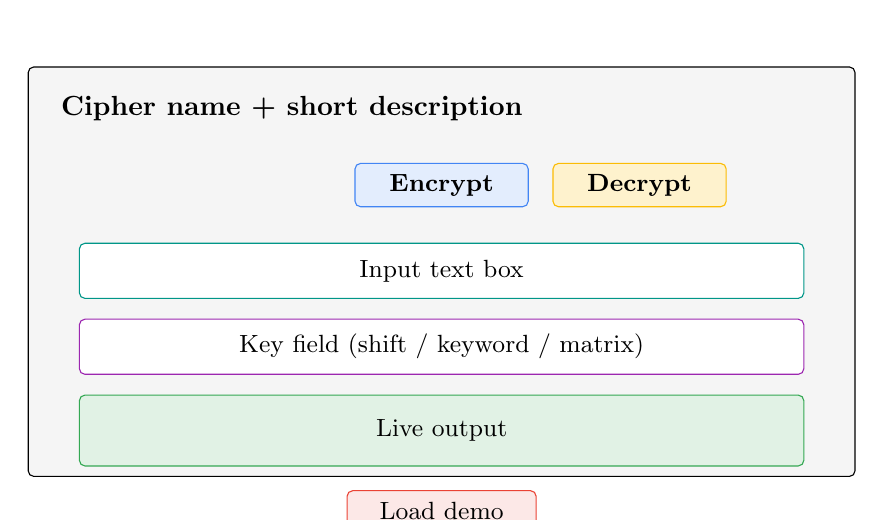
\begin{tikzpicture}[
  box/.style={draw, rounded corners=2pt, align=left, font=\small},
]
  \node[box, fill=gray!8, minimum width=10.5cm, minimum height=5.2cm] (page) {};
  \node[anchor=north west, font=\bfseries] at ([xshift=0.3cm, yshift=-0.25cm]page.north west)
    {Cipher name + short description};

  \node[box, fill=cBlue!15, draw=cBlue, minimum width=2.2cm, minimum height=0.55cm]
    at ([yshift=1.1cm]page.center) (enc) {\textbf{Encrypt}};
  \node[box, fill=cOrange!20, draw=cOrange, minimum width=2.2cm, minimum height=0.55cm, right=0.3cm of enc]
    (dec) {\textbf{Decrypt}};

  \node[box, fill=white, draw=cTeal, minimum width=9.2cm, minimum height=0.7cm, below=0.45cm of enc]
    (in) {Input text box};
  \node[box, fill=white, draw=cPurple, minimum width=9.2cm, minimum height=0.7cm, below=0.25cm of in]
    (key) {Key field (shift / keyword / matrix)};
  \node[box, fill=cGreen!15, draw=cGreen, minimum width=9.2cm, minimum height=0.9cm, below=0.25cm of key]
    (out) {Live output};
  \node[box, fill=cRed!12, draw=cRed, minimum width=2.4cm, minimum height=0.5cm, below=0.3cm of out]
    (demo) {Load demo};
\end{tikzpicture}
\end{center}

This shared UI made it easy for the team to add four tools without redesigning each page from scratch.

% ===================== 8 =====================
\section{Tools Summary}

\begin{center}
\begin{tabular}{@{}llll@{}}
\toprule
\textbf{Tool} & \textbf{Key} & \textbf{Works on} & \textbf{Special handling} \\
\midrule
Caesar & Shift number & Single letters & Keeps case \& non-letters \\
Vigen\`{e}re & Keyword & Single letters & Keyword skips non-letters \\
Playfair & Keyword & Letter pairs & \(5\times5\) square, I/J merge, \(X\) pad \\
Hill & \(n\times n\) matrix & Blocks of \(n\) & Must be invertible mod 26 \\
\bottomrule
\end{tabular}
\end{center}

\section{Team Work}

We worked as a team of four. Together we:
\begin{itemize}[leftmargin=*]
  \item Chose the four ciphers from the course syllabus.
  \item Implemented encrypt/decrypt logic in JavaScript modules.
  \item Built the web pages (input, key, mode, output, demo).
  \item Tested each tool with sample messages and edge cases (spaces, odd length, bad Hill matrix).
\end{itemize}

% ===================== 9 =====================
\section{Conclusion}

We built four working classical cipher tools---Caesar, Vigen\`{e}re, Playfair, and Hill---as a course project. Each tool has a simple UI and real JavaScript code that runs in the browser. The project helped us connect class formulas to something we can click, type into, and demonstrate.

\end{document}
